\documentclass[11pt,spanish,a4paper]{article}
% Versión 1.er cuat 2017 Víctor Bettachini < bettachini@df.uba.ar >

\usepackage{babel}
\addto\shorthandsspanish{\spanishdeactivate{~<>}}
\usepackage[utf8]{inputenc}
\usepackage{float}

\usepackage{units}
\usepackage[separate-uncertainty=true, multi-part-units=single, locale=FR]{siunitx}

\usepackage{amsmath}
\usepackage{amstext}
\usepackage{amssymb}

% \usepackage{enumerate}

\newcommand{\pvec}[1]{\vec{#1}\mkern2mu\vphantom{#1}}

\usepackage{tikz}
\usepackage{xparse}
\usetikzlibrary{calc}

\tikzset{%
    Cote node/.style={%
        midway,
        sloped,
        fill=white,
        inner sep=1.5pt,
        outer sep=2pt
    },
    Cote arrow/.style={%
        <->,
        >=latex,
        very thin
    }
}

\makeatletter
\NewDocumentCommand{\Cote}{%
    s       % cotation avec les flèches à l'extérieur
    D<>{1.5pt} % offset des traits
    O{.75cm}    % offset de cotation
    m       % premier point
    m       % second point
    m       % étiquette
    D<>{o}  % () coordonnées -> angle
            % h -> horizontal,
            % v -> vertical
            % o or what ever -> oblique
    O{}     % parametre du tikzset
    }{%

    {\tikzset{#8}

    \coordinate (@1) at #4 ;
    \coordinate (@2) at #5 ;

    \if #7v % Cotation verticale
        \coordinate (@0) at ($($#4!.5!#5$) + (#3,0)$) ; 
        \coordinate (@4) at (@0|-@1) ;
        \coordinate (@5) at (@0|-@2) ;
    \else
    \if #7h % Cotation horizontale
        \coordinate (@0) at ($($#4!.5!#5$) + (0,#3)$) ; 
        \coordinate (@4) at (@0-|@1) ;
        \coordinate (@5) at (@0-|@2) ;
    \else % cotation encoche
    \ifnum\pdfstrcmp{\unexpanded\expandafter{\@car#7\@nil}}{(}=\z@
        \coordinate (@5) at ($#7!#3!#5$) ;
        \coordinate (@4) at ($#7!#3!#4$) ;
    \else % cotation oblique    
        \coordinate (@5) at ($#5!#3!90:#4$) ;
        \coordinate (@4) at ($#4!#3!-90:#5$) ;
    \fi\fi\fi

    \draw[very thin,shorten >= #2,shorten <= -2*#2] (@4) -- #4 ;
    \draw[very thin,shorten >= #2,shorten <= -2*#2] (@5) -- #5 ;

    \IfBooleanTF #1 {% avec étoile
    \draw[Cote arrow,-] (@4) -- (@5)
        node[Cote node] {#6\strut};
    \draw[Cote arrow,<-] (@4) -- ($(@4)!-6pt!(@5)$) ;   
    \draw[Cote arrow,<-] (@5) -- ($(@5)!-6pt!(@4)$) ;   
    }{% sans étoile
    \ifnum\pdfstrcmp{\unexpanded\expandafter{\@car#7\@nil}}{(}=\z@
        \draw[Cote arrow] (@5) to[bend right]
            node[Cote node] {#6\strut} (@4) ;
    \else
    \draw[Cote arrow] (@4) -- (@5)
        node[Cote node] {#6\strut};
    \fi
    }}
    }
\makeatother

\usetikzlibrary{decorations.pathmorphing, patterns}

\usepackage{graphicx}
\graphicspath{{./graphs_oscilaciones/}}

\voffset-3.5cm
\hoffset-3cm
\setlength{\textwidth}{17.5cm}
\setlength{\textheight}{27cm}

\usepackage{lastpage}
\usepackage{fancyhdr}
\pagestyle{fancyplain}
\fancyhead{}
\fancyfoot{}
\fancyfoot[C]{ {\tiny Actualizado al \today} }
\fancyfoot[RO, LE]{Pág. \thepage/\pageref{LastPage}}
\renewcommand{\headrulewidth}{0pt}
\renewcommand{\footrulewidth}{0pt}


\begin{document}
\begin{center}
\textbf{Física 2} (Físicos) \hfill \textcopyright {\tt DF, FCEyN, UBA}\\
%	\textsc{\large Física 2 (Físicos)} - Prof. Diana Skigin - 2"o cuat. 2014\\
%	\textsc{\large Primer Cuatrimestre - 2014}\\
	\textsc{\LARGE Oscilacioes libres y forzadas}
	% \textsc{\large Guía 1:} Oscilaciones libres y forzadas
\end{center}


\begin{enumerate}

\section*{Oscilador armónico de un único grado de libertad}

\item Escriba y resuelva las ecuaciones de movimiento asociadas con los
siguientes sistemas: 
\begin{enumerate}
\item Péndulo de longitud $l$ en presencia de un campo gravitatorio de
constante $g$. Discuta todas las aproximaciones que realiza.
\item Oscilaciones longitudinales de una masa $m$ sujeta a dos paredes
mediante dos resortes iguales de constante $k$; para los dos casos: 

\begin{enumerate}
\item longitud natural del resorte $l_{0}$ $(l_{0}<l)$, y 
\item ``slinky'' $(l_{0}=0)$. 
\end{enumerate}
\item Oscilaciones transversales del sistema del punto anterior, discutiendo
las diferencias entre los casos 1) y 2), y analizando cuidadosamente
las aproximaciones que realiza. En el caso 1) analice la diferencia
entre considerar que los resortes están tensionados en la posición
de equilibrio $(l_{0}<l)$ o que están relajados en dicha posición
$(l_{0}=l)$.
\begin{figure}[H]
\centering{}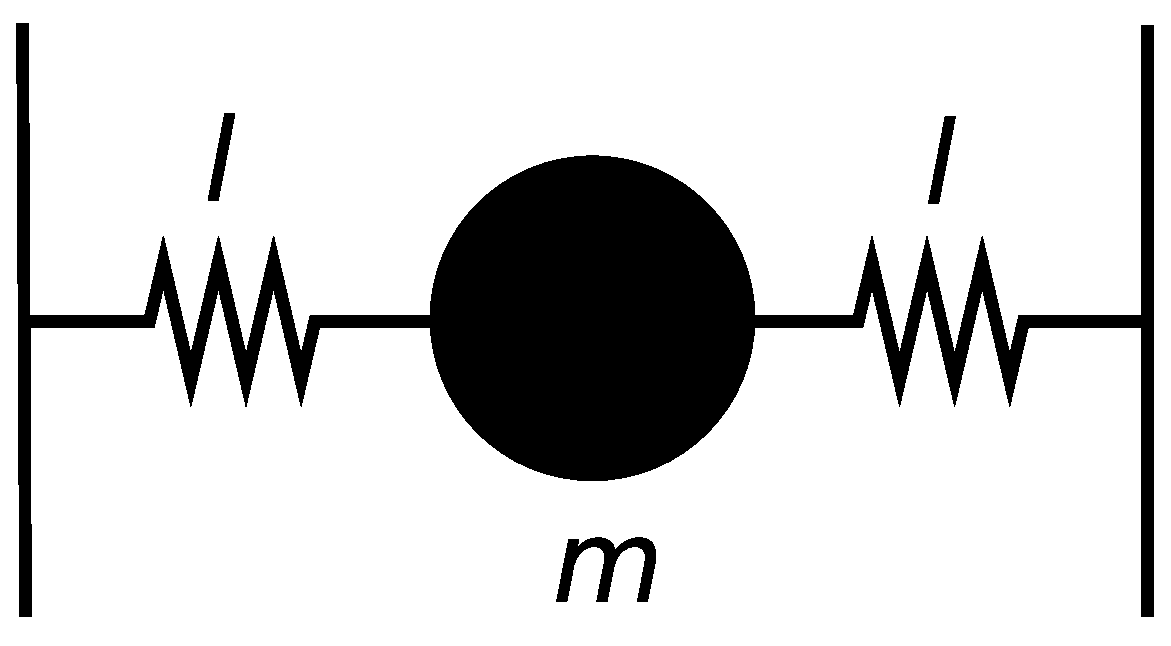
\includegraphics[clip,scale=0.25]{ej1-1}
\end{figure}

\end{enumerate}


\subsection*{Oscilador armónico amortiguado}

\item Considere el movimiento de una masa $m$ sujeta a un resorte de constante
elástica $K=m\omega_{0}^{2}$ y constante de amortiguamiento por unidad
de masa $\Gamma$. \\
Demuestre que el resultado para el oscilador ``sobreamortiguado''
dado por
\[
x(t)=\mathrm{e}^{-\Gamma t/2}\left\{ x(0)\cosh\left(\left|\omega\right|t\right)+\left[\dot{x}(0)+\frac{1}{2}\Gamma x(0)\right]\frac{\senh\left(\left|\omega\right|t\right)}{\left|\omega\right|}\right\} 
\]
se deduce de las siguientes
\[
x(t)=\mathrm{e}^{-\Gamma t/2}\left\{ x(0)\cos\left(\omega t\right)+\left[\dot{x}(0)+\frac{1}{2}\Gamma x(0)\right]\frac{\sen\left(\omega t\right)}{\omega}\right\} 
\]
\[
\omega=\pm i\left|\omega\right|,\,\,\,\left|\omega\right|=\sqrt{\frac{1}{4}\Gamma^{2}-\omega_{0}^{2}}
\]
\textbf{Sugerencia}: verifique primero las identidades $\cos\left(ix\right)=\cosh\left(x\right)$
y $\sen\left(ix\right)=i\senh\left(x\right)$; luego úselas.



\item Comenzando con la ecuación general dada en el problema anterior para
oscilaciones libres subamortiguadas, muestre que para amortiguamiento
crítico la solución es:
\[
x(t)=\mathrm{e}^{-\Gamma t/2}\left\{ x(0)+\left[\dot{x}(0)+\frac{1}{2}\Gamma x(0)\right]t\right\} 
\]
Muestre que también se obtiene este resultado comenzando con la ecuación
para oscilaciones sobreamortiguadas.


\subsection*{Oscilador armónico forzado}


\item% \quad{}
\begin{enumerate}
\item Escriba la ecuación de movimiento para una masa $m$ sujeta a un resorte
de constante elástica $k$ y constante de amortiguamiento por unidad
de masa $\Gamma$, sobre la que se realiza una fuerza dependiente
del tiempo $F(t)$. 
\item Proponga la siguiente solución homogénea: $x_{h}(t)=C\mathrm{e}^{-t/2\tau}\cos\left(\omega_{1}t+\theta\right)$
y halle los valores de $\tau$ y de $\omega_{1}$. ¿De qué depende
el valor de $C$ y de $\theta$? ¿Es lícito plantear las condiciones
iniciales sobre la solución homogénea? 
\item Considere que $F(t)$ tiene la forma $F(t)=F_{0}\cos\left(\omega t\right)$
(discuta si se pierde generalidad al suponer que la fuerza externa
tiene esa forma) y proponga la siguiente solución particular: $x_{p}(t)=A\sen\left(\omega t\right)+B\cos\left(\omega t\right)$.
Obtenga $A$ y $B$. Grafique cualitativamente $A$ y $B$ en función
de $\omega$. 
\item Grafique cualitativamente la posición de la masa en función del tiempo. 
\item Calcule la potencia media que se consume en el estado estacionario
y la potencia media de pérdida por fricción. Verifique la igualdad
de ambas potencias. 
\item Verifique que si $x_{1}(t)$ es solución de la ecuación diferencial
cuando la fuerza externa es $F_{1}(t)$ y $x_{2}(t)$ lo es cuando
la fuerza externa es $F_{2}(t)$, entonces $x(t)=x_{1}(t)+x_{2}(t)$
será solución de la ecuación diferencial cuando la fuerza externa
sea $F(t)=F_{1}(t)+F_{2}(t)$ si y sólo si las condiciones iniciales
son la suma de las condiciones iniciales de los dos casos. 
\item Proponga ahora como solución particular la solución compleja $x_{p}(t)=A\mathrm{e}^{-i\omega t}$
	y demuestre que $\Re\mathfrak{e}(A)=A_{\mathrm{el\acute{a}stico}}$ y que $\Im\mathfrak{m}(A)=A_{\mathrm{absorbente}}$.
¿Por qué es así?
\end{enumerate}
\item Sea un oscilador armónico con una frecuencia de oscilación $\nu_{0}=10\mbox{\,\ Hz}$
y con un tiempo de decaimiento muy largo. Si este oscilador es alimentado
con una fuerza armónicamente oscilante y con una frecuencia de 10
Hz, adquirirá una gran amplitud, es decir, ``resonará'' en la frecuencia
de excitación. Ninguna otra fuerza motriz oscilante en forma armónica
producirá una gran amplitud (una resonancia). 

\begin{enumerate}
\item Justifique el enunciado anterior. 
\item Luego suponga que el oscilador está sujeto a una fuerza que es una
pulsación cuadrada repetida periódicamente y cuya duración es $0.01$
s repetida una vez por segundo. Describa cualitativamente el análisis
de Fourier de la pulsación cuadrada repetitiva. 
\item ¿``Resonará'' el oscilador armónico (adquirirá una gran amplitud)
bajo la influencia de esta fuerza motriz? 
\item Suponga que la fuerza motriz es la misma pulsación cuadrada (de ancho
$0.01$ s) pero repetida dos veces por segundo. ¿Resonará el oscilador?
Responder a la misma pregunta para velocidades de repetición de 3
a 9 segundos.
\end{enumerate}


\section*{Sistemas de N grados de libertad}

\item %\qquad{}
\begin{figure}[H]
\centering{}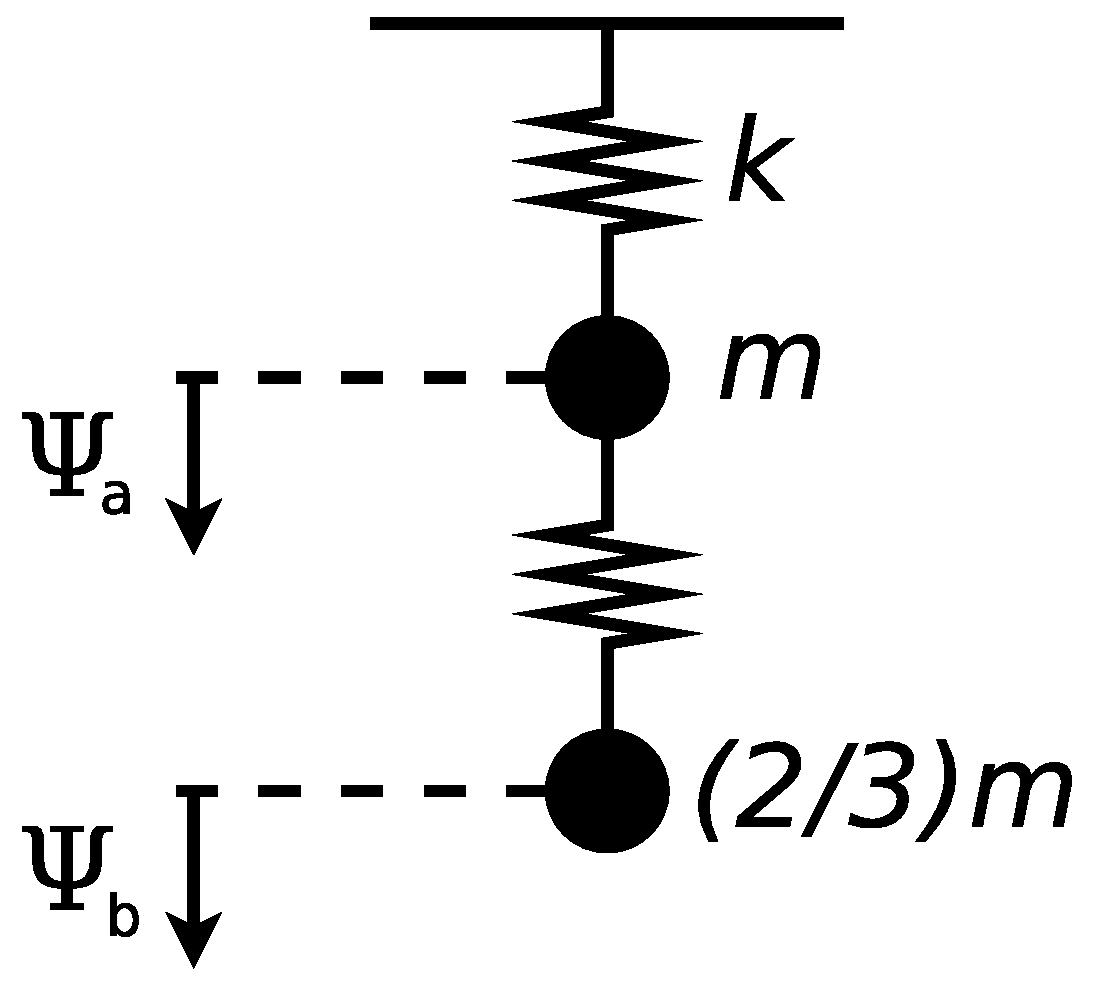
\includegraphics[clip,scale=0.25]{ej1-6}
\end{figure}
\begin{enumerate}
\item Considere el sistema de la figura en ausencia de gravedad y obtenga
sus frecuencias naturales de oscilación y los modos normales correspondientes.
Escriba las ecuaciones de movimiento de cada masa.
\item Sabiendo que a $t=0$ el sistema satisface las siguientes condiciones:
$\Psi_{a}(0)=1,\,\Psi_{b}(0)=0$ y que se encuentra en reposo, encuentre
el movimiento de cada partícula. 
\item Analice cómo se modifica el resultado por la presencia de la gravedad.
\end{enumerate}



\subsection*{Pulsaciones entre modos normales}

\item Considere el sistema de dos péndulos de igual longitud $l$ pero de
masas diferentes $m_{a}$ y $m_{b}$, acoplados mediante un resorte
de constante $k$. 
\begin{figure}[H]
\centering{}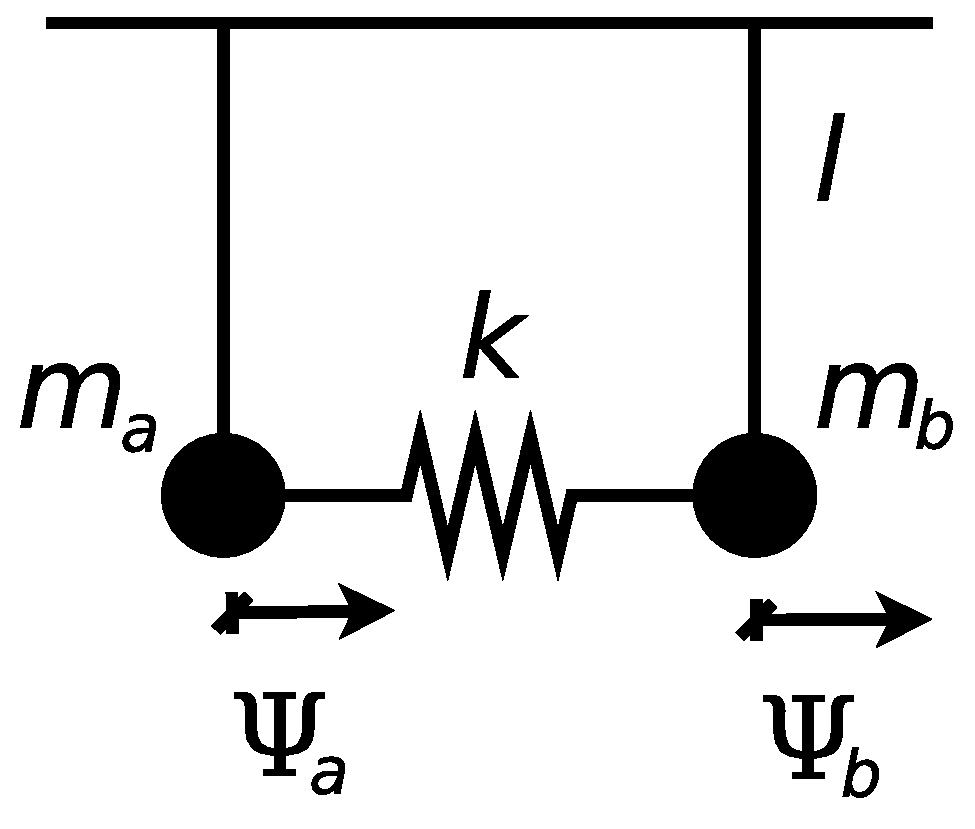
\includegraphics[clip,scale=0.3]{ej1-7}
\end{figure}


\begin{enumerate}
\item Escriba las ecuaciones de movimiento de cada masa. 
\item Obtenga las frecuencias naturales del sistema y sus modos normales
de oscilación. Interprete el significado físico de estos modos normales. 
\item Suponiendo que el acoplamiento es débil, es decir: $k\ll\frac{g}{l}\frac{m_{a}m_{b}}{m_{a}+m_{b}}$,
y que las condiciones iniciales son $\dot{\Psi}_{a}(0)=0,\dot{\Psi}_{b}(0)=0,\Psi_{a}(0)=0,\Psi_{b}(0)=1$;
obtenga el movimiento de cada masa y grafíquelo en función del tiempo. 
\item Calcule los valores medios, en un ciclo rápido, de $T_{a}$ y $T_{b}$,
donde $T$ indica energía cinética. Grafique $\left\langle T_{a}\right\rangle $
y $\left\langle T_{b}\right\rangle $, y analice las diferencias en
el gráfico como función de las diferencias entre las masas ($m_{a}=m_{b}$
y $m_{a}$ muy diferente de $m_{b}$). Calcule el valor medio de la
energía de interacción entre las dos partículas.
\end{enumerate}


\item Considere el sistema de la figura. Las masas están apoyadas en una
mesa sen rozamiento, sujetas a las paredes por resortes de constante
$k$ y unidas por otro resorte de constante $k'$. 
\begin{figure}[H]
\centering{}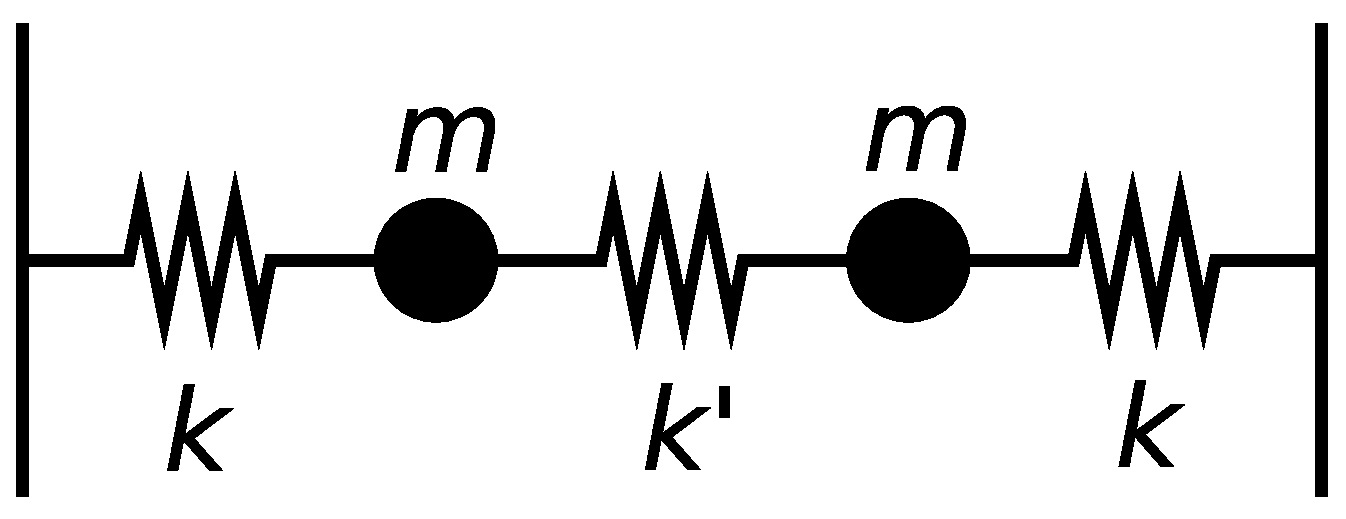
\includegraphics[clip,scale=0.25]{ej1-8}
\end{figure}
\begin{enumerate}
\item Obtenga las frecuencias y los modos transversales del sistema. 
\item ¿Bajo qué condiciones espera observar batidos? ¿Qué son los batidos?
\end{enumerate}



\subsection*{Excitación selectiva de modos | Condiciones iniciales}


\item Considere el sistema simplificado de la figura que se basa en una
molécula triatómica simétrica. En el equilibrio dos átomos de masa
$m$ están situados a ambos lados del átomo de masa $M=2m$ y vinculados
por resortes de constante $k$ y longitud natural $l_{0}$. Como sólo
estamos interesados en analizar los modos longitudinales, supondremos
que las masas se encuentran dentro de una canaleta que impide todo
tipo de movimiento en la dirección transversal. 
\begin{figure}[H]
\centering{}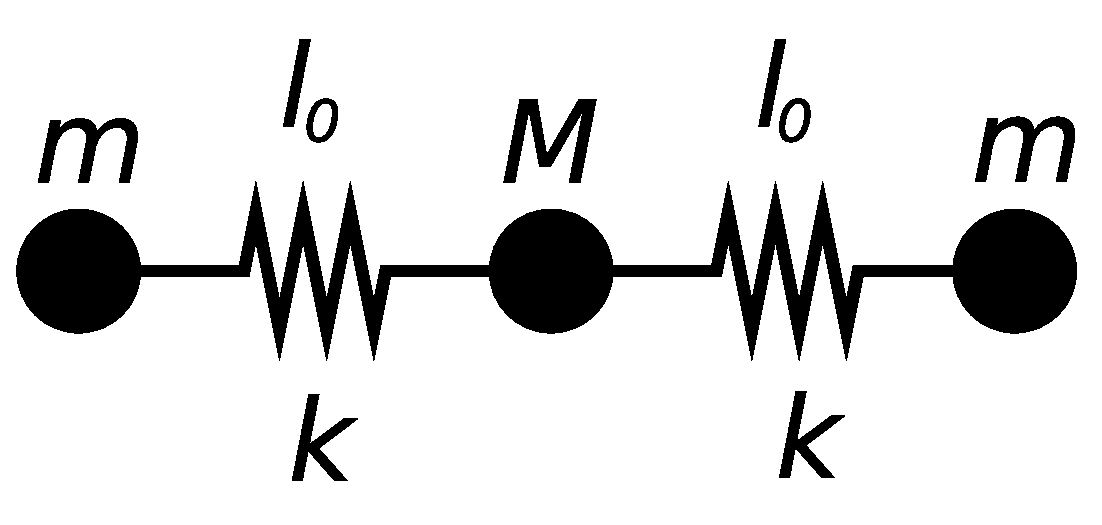
\includegraphics[clip,scale=0.25]{ej1-9}
\end{figure}


\begin{enumerate}
\item Encuentre las ecuaciones de movimiento de cada masa. 
\item Halle las frecuencias de los modos normales. 
\item Dibuje las configuraciones de cada modo. 
\item Establezca cuáles deben ser las condiciones iniciales para excitar
sólo el modo más alto (mayor frecuencia).
\end{enumerate}


\item Considere el sistema de la figura, en la que los resortes verticales
tienen longitud natural $l_{0}$ y constante $k_{1}$, y los horizontales
$a_{0}=0$ (``slinkies'') y $k_{2}$.
\begin{figure}[H]
\centering{}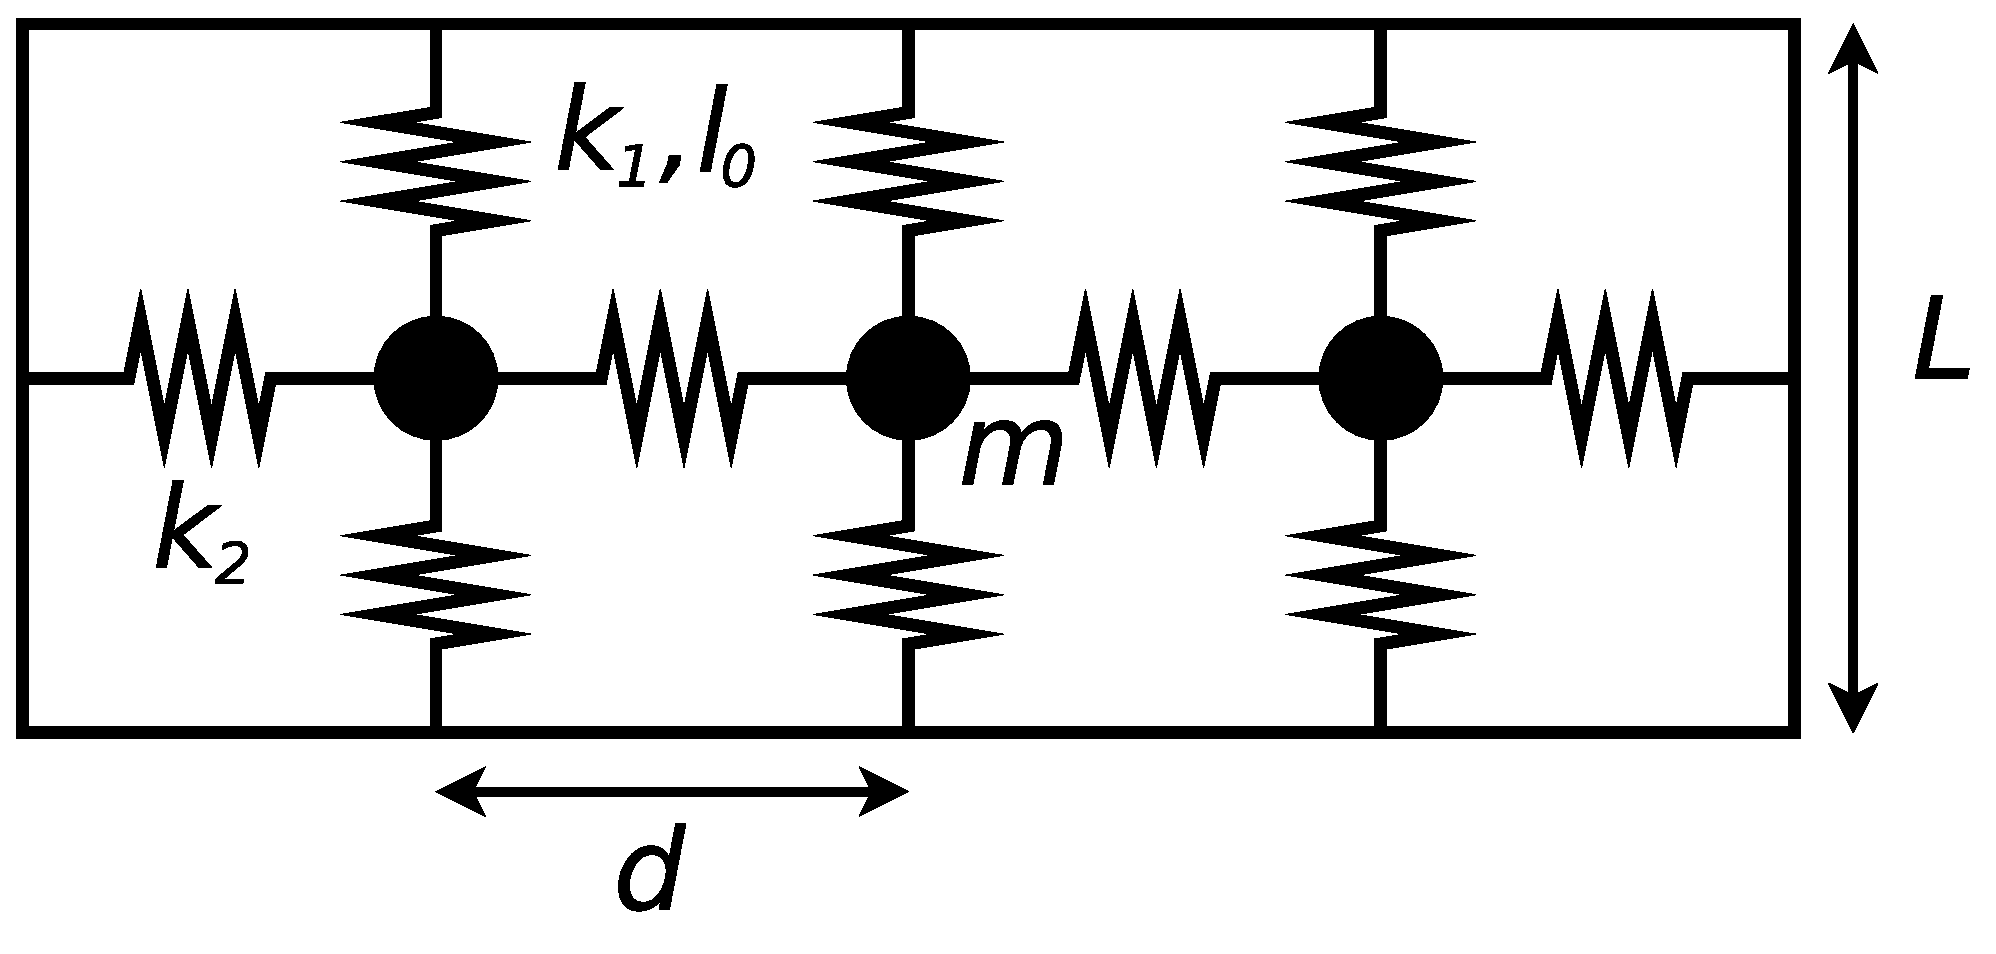
\includegraphics[clip,scale=0.25]{ej1-10}
\end{figure}
\begin{enumerate}
\item Calcule las frecuencias propias y los modos normales. 
\item Considere que las condiciones iniciales son tales que el sistema oscila
horizontalmente, estando su movimiento descripto por una superposición
de los dos primeros modos. Halle la energía cinética de cada masa
y la energía potencial del sistema, el promedio temporal de las mismas
y la frecuencia de pulsación $\omega_{p}$. \end{enumerate}
\begin{description}
\item [{Datos:}] $l_{0}$, $k_{1}$, $a_{0}=0$, $k_{2}$, $L$, $d$,
$m$.
\end{description}


\section*{Modos normales en sistemas periódicos}


\item Considere el sistema de $N$ masas mostrado en la figura. 
\begin{figure}[H]
\begin{centering}
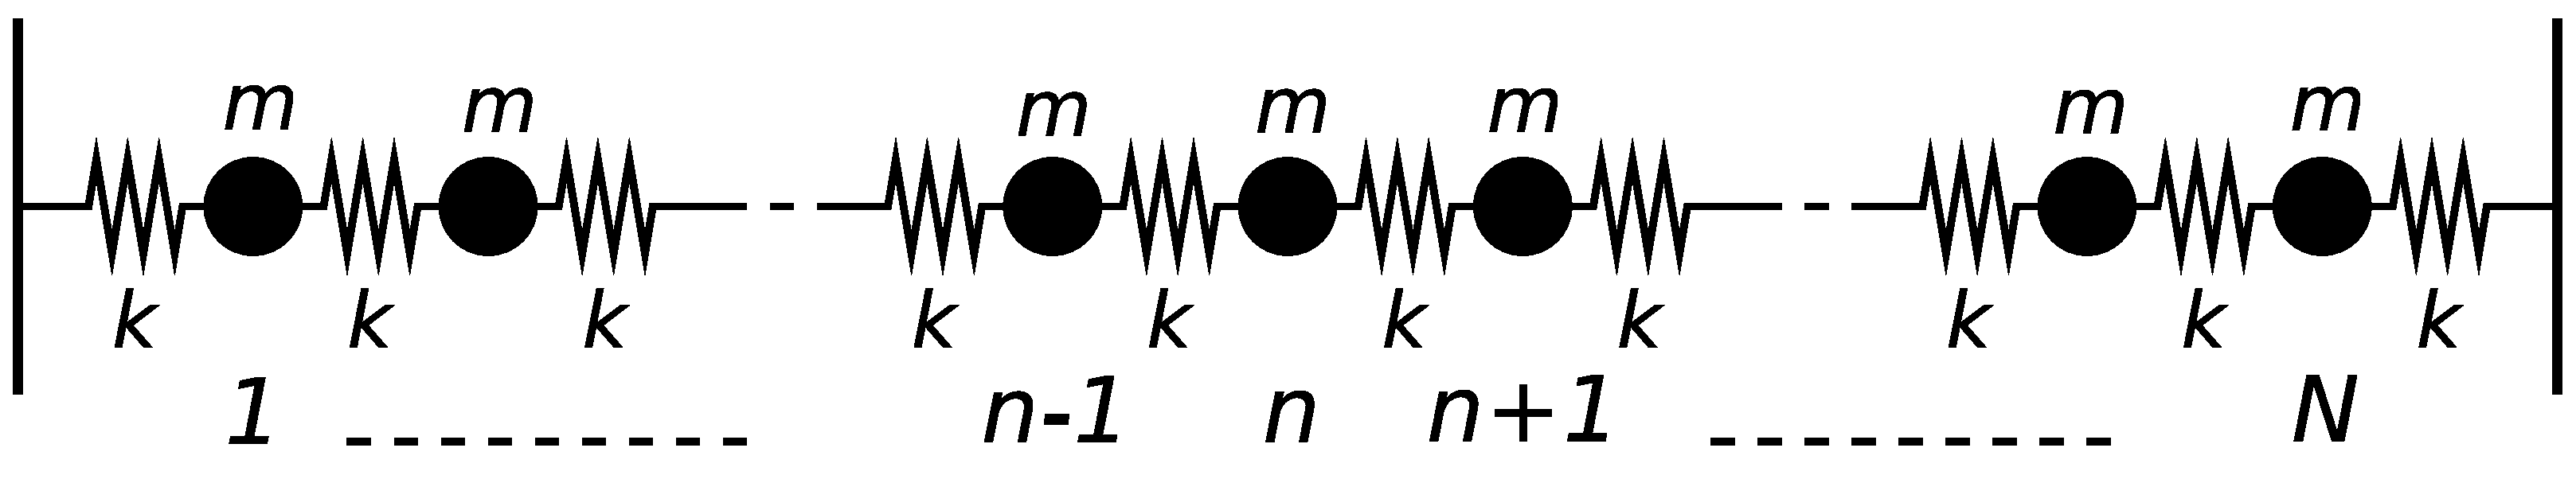
\includegraphics[clip,scale=0.25]{ej1-11}
\par\end{centering}

\end{figure}


\begin{enumerate}
\item Usando la aproximación de pequeños ángulos, escriba la ecuación de
movimiento transversal para la partícula enésima. 
\item Proponga una solución de la forma:
\[
\Psi_{n}^{(p)}(t)=A^{(p)}\cos\left(nk^{(p)}a+\alpha^{(p)}\right)\cos\left(\omega^{(p)}t+\phi^{(p)}\right)
\]
Halle la relación de dispersión y grafíquela. ¿Depende esta relación
de las condiciones de contorno? ¿Cuánto vale la frecuencia más baja?
¿Qué representa dicho modo? 
\item Obtenga las frecuencias correspondientes a los modos normales cuando
ambos extremos están libres (atención: ¿cómo sería un ``extremo libre''
en esta configuración?) y escriba la solución general para la masa
enésima. 
\item Ídem. anterior, pero considerando que el extremo izquierdo está libre
y el derecho fijo a la pared. 
\item Particularice los resultados de los dos ítems anteriores para el caso
en que $N=3$.
\end{enumerate}



\item Considere el sistema de péndulos acoplados de la figura. 
\begin{figure}[H]
\centering{}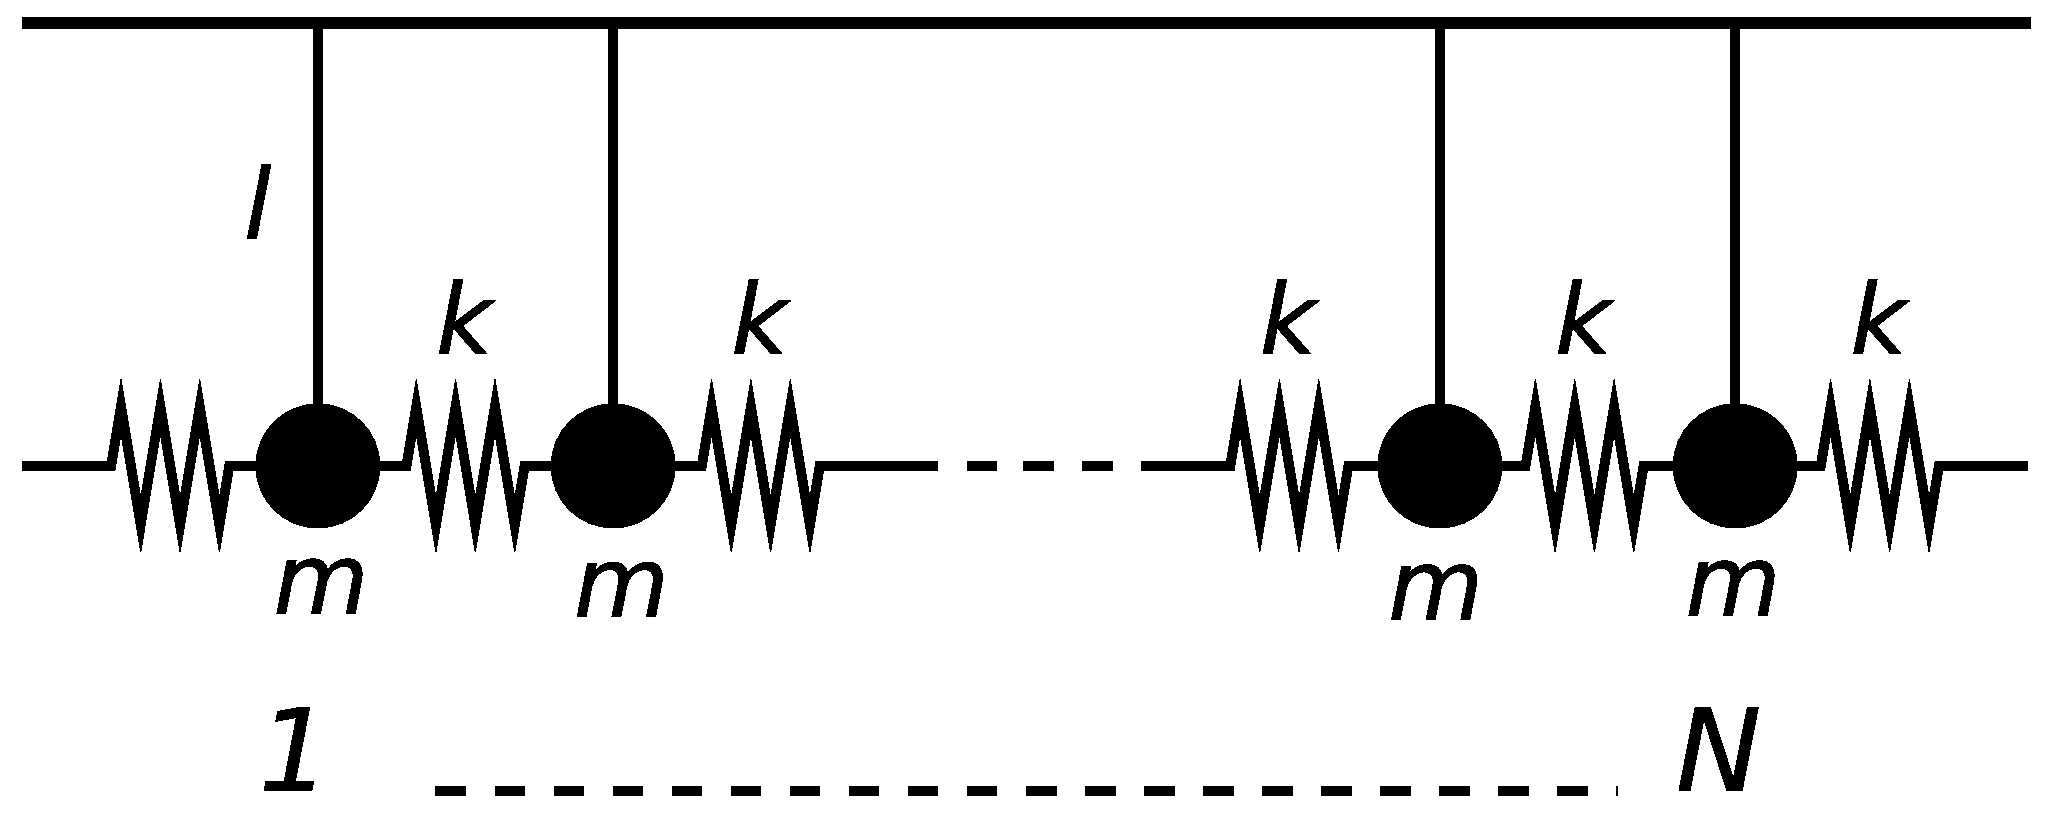
\includegraphics[clip,scale=0.25]{ej1-12}
\end{figure}
\begin{enumerate}
\item Escriba la ecuación de movimiento. Proponga una solución semejante
a la del problema anterior y halle la relación de dispersión. Compárela
con la obtenida en el problema anterior. ¿Cuánto vale la frecuencia
más baja? ¿Qué representa dicho modo? 
\item Obtenga las frecuencias correspondientes a los modos normales cuando
los resortes de los extremos están fijos y dé las condiciones iniciales
para excitar el primer armónico. 
\item Ídem anterior, pero para el caso en que uno de los resortes de los
extremos está libre. 
\end{enumerate}


\subsection*{Oscilaciones forzadas de sistemas con N grados de libertad}


\item Considere el sistema de dos péndulos acoplados, tal que uno de ellos
es impulsado por una fuerza $F=F_{0}\cos(\Omega t)$. Desprecie el
amortiguamiento. Muestre que:
\[
\Psi_{a}\approx\frac{F_{0}}{2M}\cos(\Omega t)\left[\frac{1}{\omega_{1}^{2}-\Omega^{2}} - \frac{1}{\omega_{2}^{2}-\Omega^{2}}\right];
\]
\[
\Psi_{b}\approx\frac{F_{0}}{2M}\cos(\Omega t)\left[\frac{1}{\omega_{1}^{2}-\Omega^{2}} + \frac{1}{\omega_{2}^{2}-\Omega^{2}}\right];
\]
\[
\frac{\Psi_{b}}{\Psi_{a}}\approx\frac{\omega_{2}^{2}-\omega_{1}^{2}}{\omega_{2}^{2}+\omega_{1}^{2}-2\Omega^{2}};
\]
donde $\omega_{1}$ es la menor de las frecuencias modales, $\omega_{2}$
es la mayor y $\Omega$ es la frecuencia de excitación.



\item Considere el sistema de 3 péndulos acoplados que se muestra en la
figura.
\begin{figure}[H]
\centering{}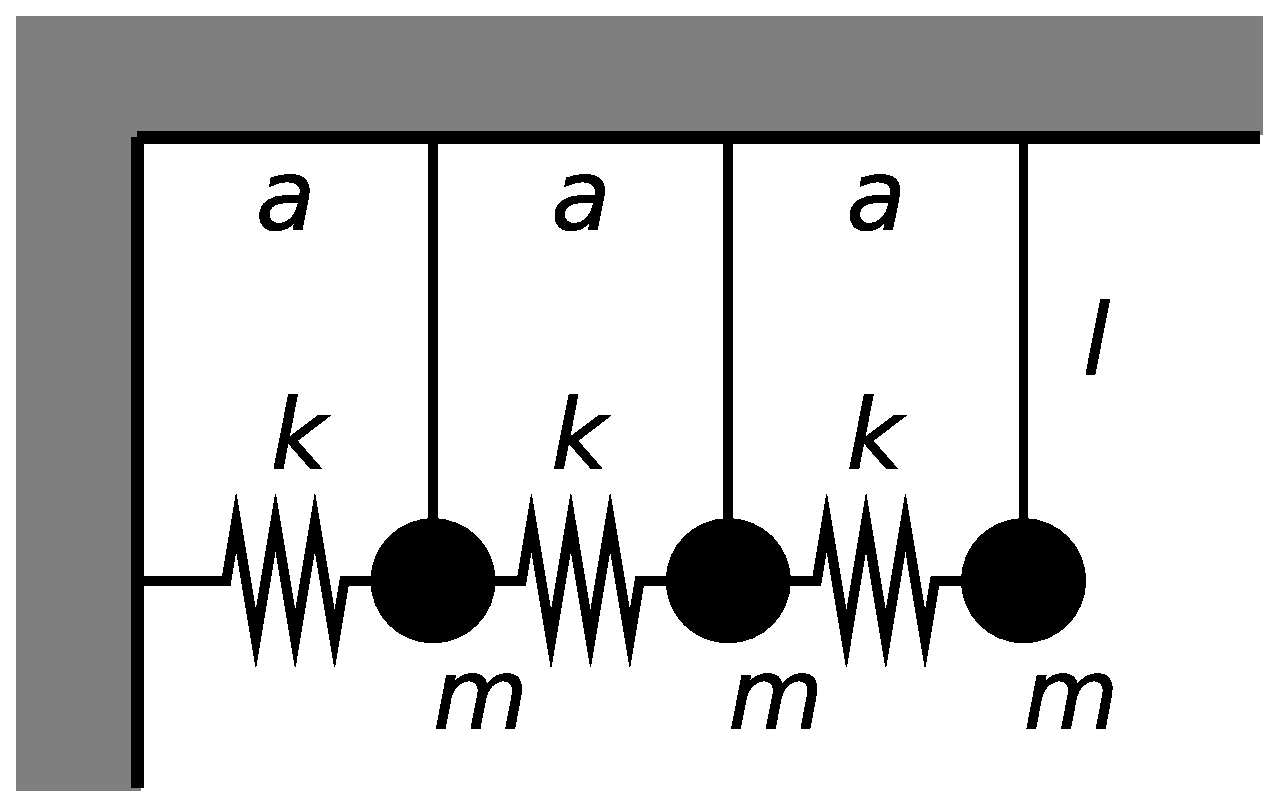
\includegraphics[clip,scale=0.25]{ej1-14}
\end{figure}

\begin{enumerate}
\item Escriba la ecuación de movimiento para cada masa y encuentre las frecuencias
propias y los modos normales del sistema. 
\item Suponga que en el extremo libre se aplica una fuerza $F=F_{0}\cos(\omega t)$.
Escriba la ecuación de movimiento para cada masa y encuentre la solución
estacionaria para cada modo. ¿Cuáles son las frecuencias de resonancia?
\end{enumerate}



\subsection*{Oscilaciones forzadas de sistemas períodicos}


\item Considere un arreglo lineal de péndulos acoplados excitados cuyo extremo
inferior está en $z=0$ y unidos a una pared rígida en $z=L$, como
se muestra en la figura.
\begin{figure}[H]
\centering{}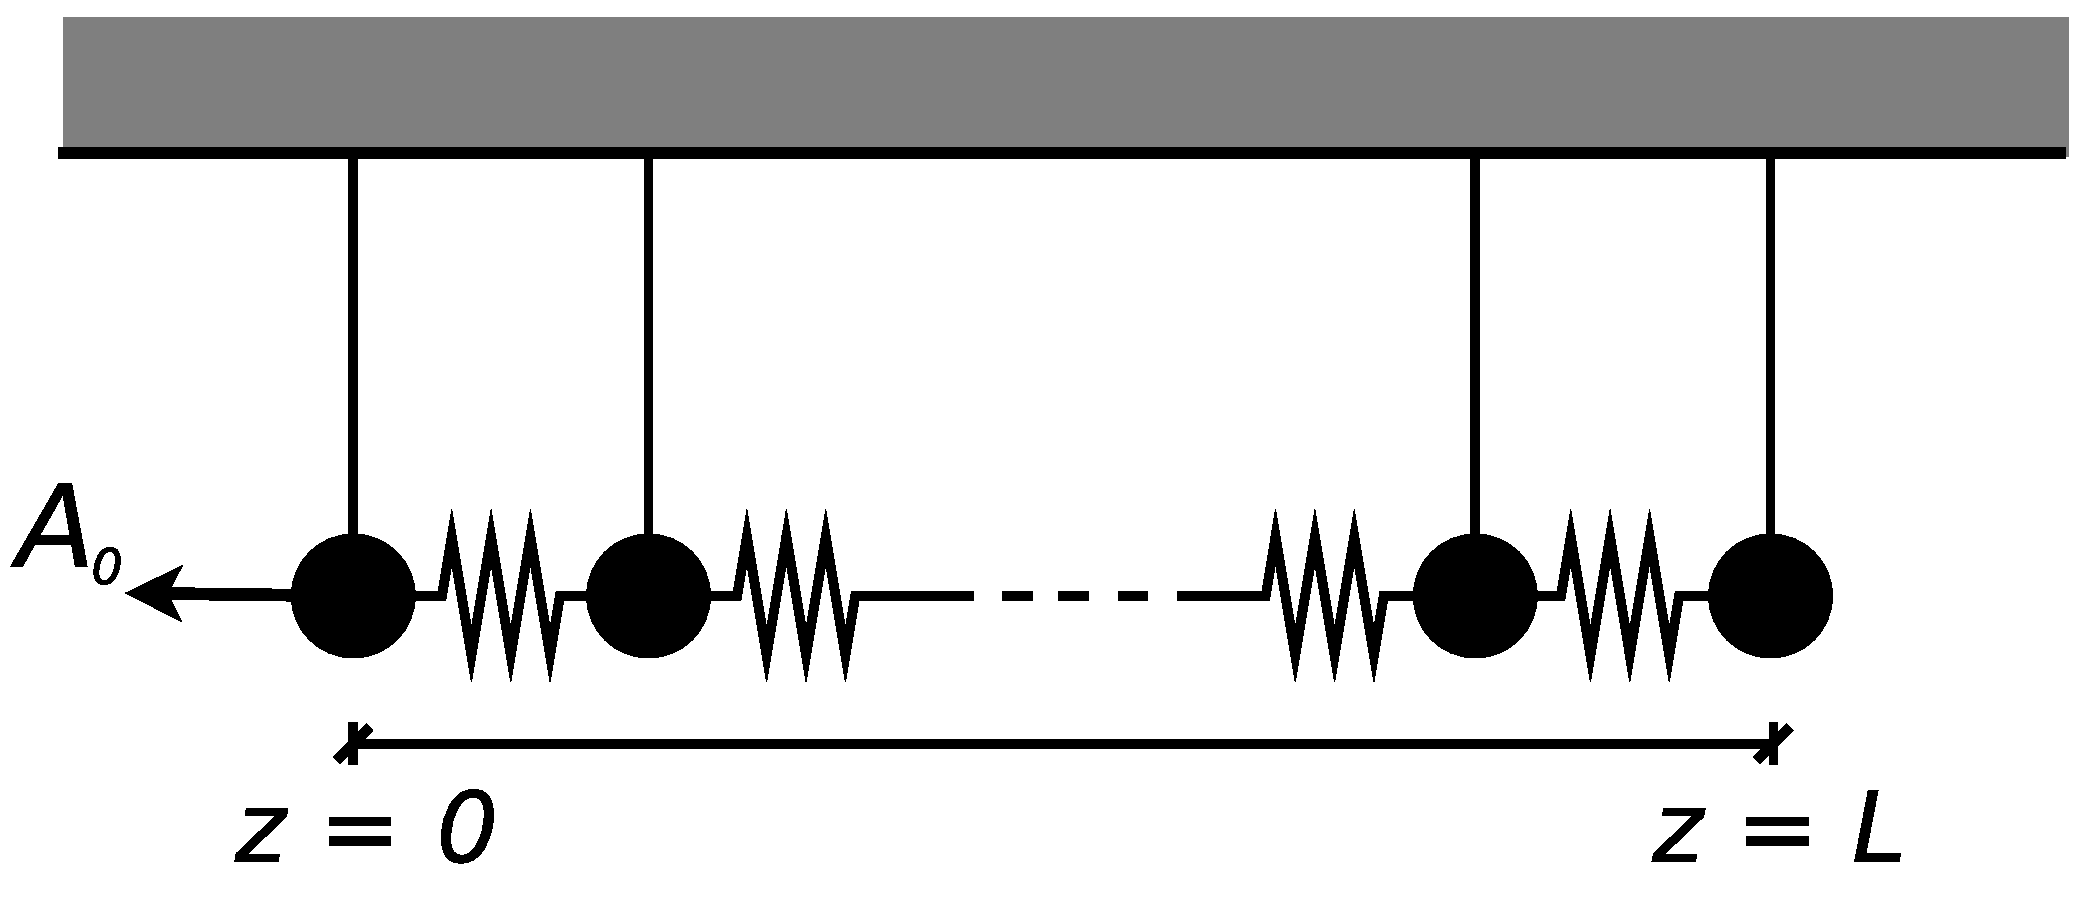
\includegraphics[clip,scale=0.25]{ej1-15}
\end{figure}
 Se aplica una fuerza externa en función del tiempo a la primera masa
($z=0$), de forma tal que se conoce su amplitud $\Psi(0,t)=A_{0}\cos(\Omega t)$.
Halle el movimiento estacionario del sistema y discuta las hipótesis
que hace. Compare con el caso de extremo derecho fijo a una pared
(o sea: agregando un resorte a la derecha de la última masa y uniéndolo
a la pared). 
\item Considere un sistema de péndulos acoplados con un cambio brusco en
$\omega_{0}^{2}$ en $z=L$, según se esquematiza en la figura. Halle
el movimiento estacionario del sistema y discuta las hipótesis que
hace.
\begin{figure}[H]
\centering{}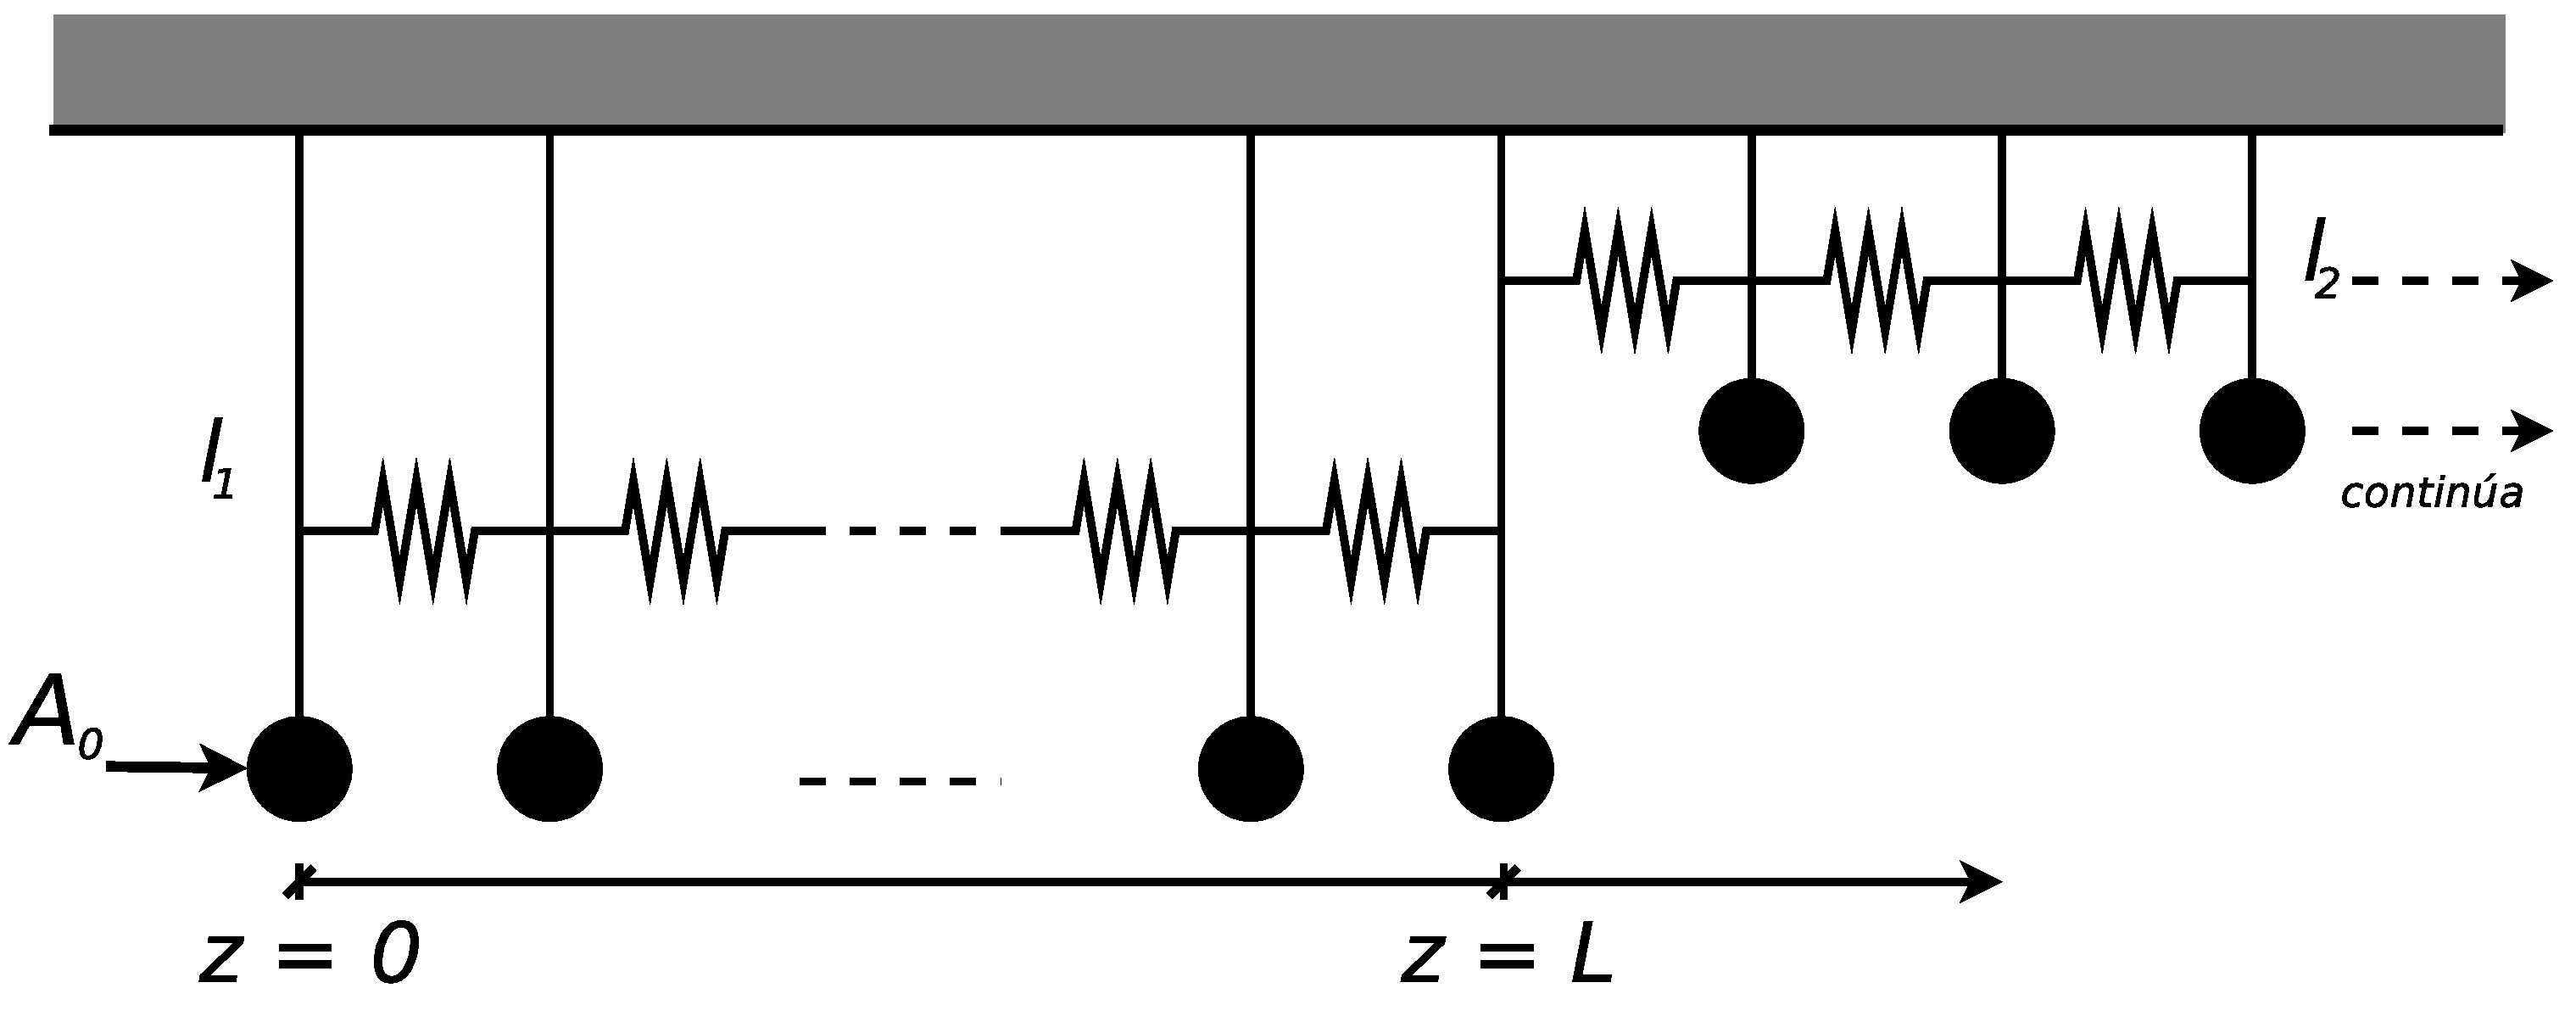
\includegraphics[clip,scale=0.25]{ej1-16}
\end{figure}


\item Para el sistema esquematizado en la figura, calcule $\Psi_{n}(t)$,
si $\Omega<\omega_{min}$.
\begin{figure}[H]
\centering{}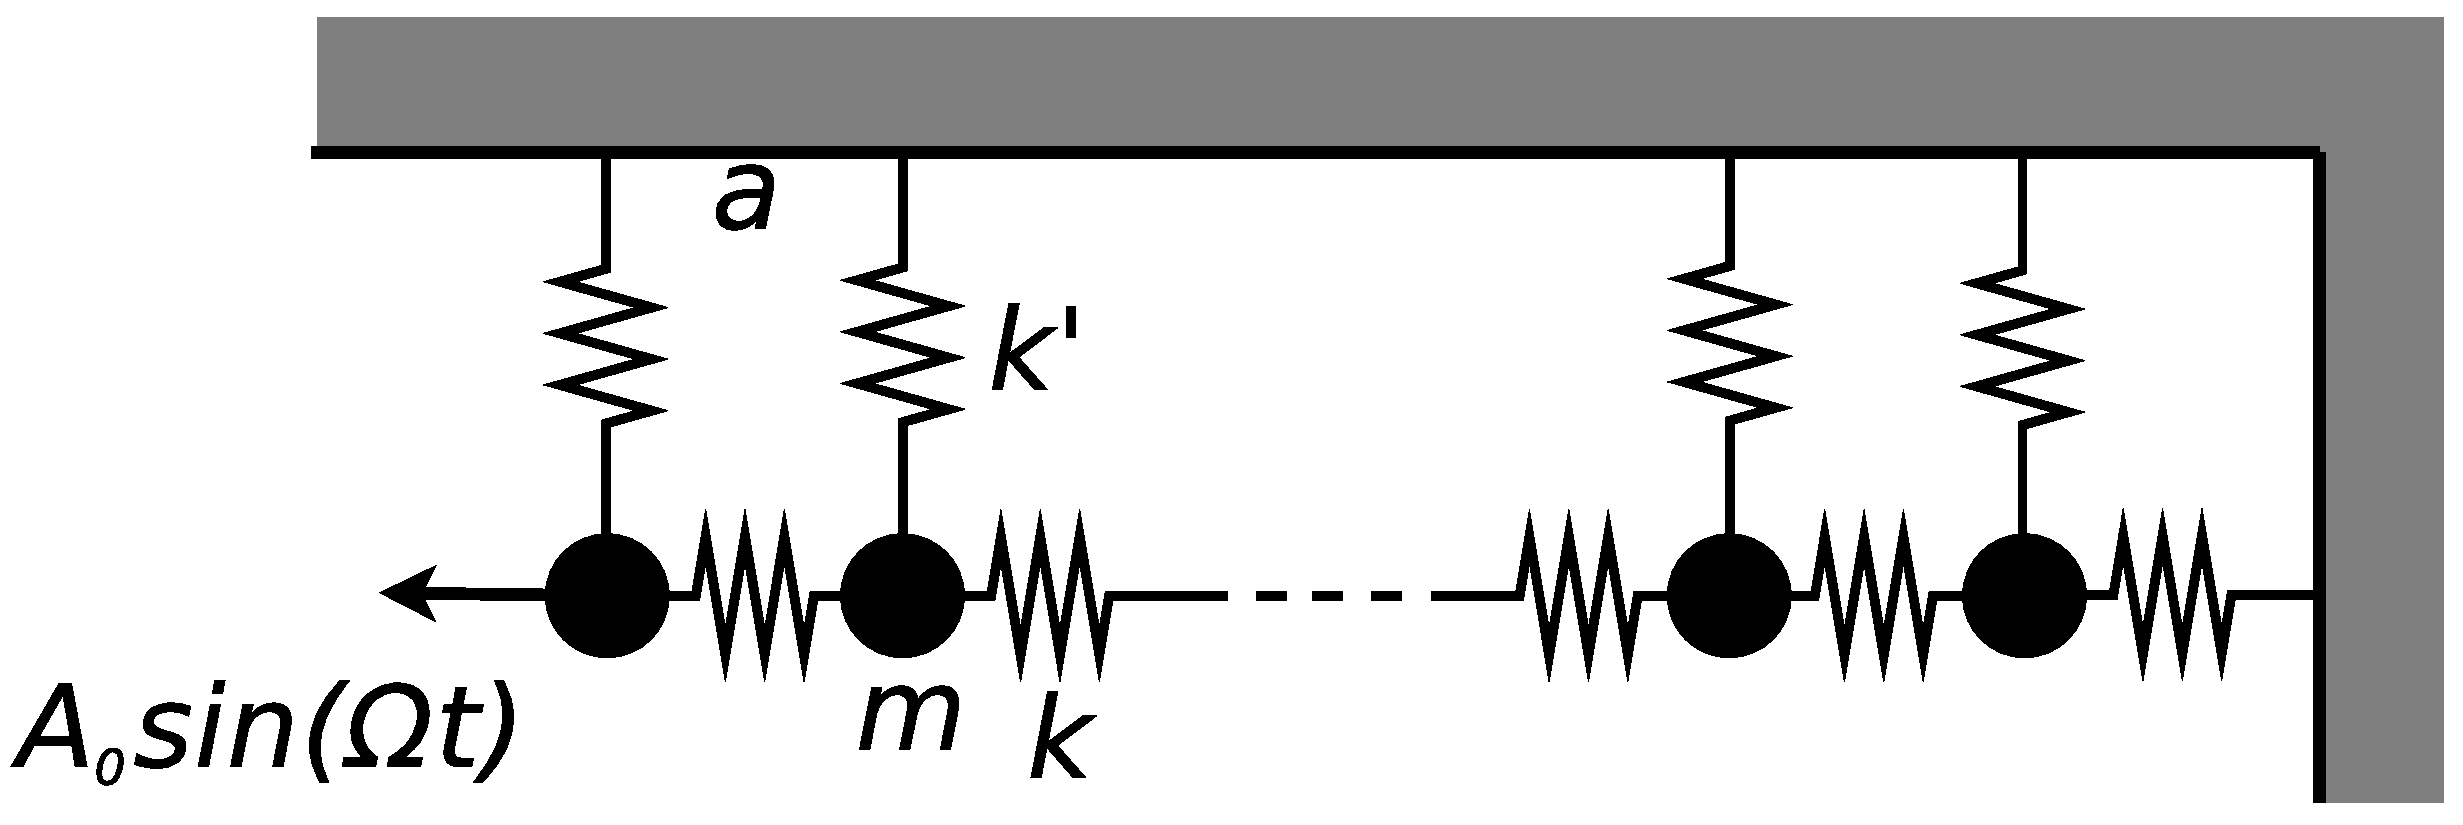
\includegraphics[clip,scale=0.25]{ej1-17}
\end{figure}



\section*{Sistemas continuos}

\subsection*{Modos normales de una cuerda}

\item Se tiene una cuerda de longitud $L$ y densidad lineal de masa $\mu$
sometida a una tensión $T_{0}$. Proponga como solución de la ecuación
de ondas para un modo normal a la expresión: $\Psi(x,t)=A\sen\left(kx+\varphi\right)\cos\left(\omega t+\theta\right)$.
Tome el sistema de coordenadas con $x=0$ en un extremo de la cuerda
y $x=L$ en el otro. Encuentre la forma particular que adopta la solución
propuesta en los siguientes casos: 

\begin{enumerate}
\item $\Psi(0,t)=\Psi(L,t)=0$ (ambos extremos están fijos). 
\item $\Psi(0,t)=0$ y $\frac{\partial\Psi}{\partial x}(L,t)=0$ (un extremo
está fijo y el otro está libre). ¿Imponer que un extremo se encuentre
``libre'' es equivalente a no imponer condiciones de contorno sobre
ese extremo? ¿Cómo lograría un extremo ``libre'' para la cuerda? 
\item $\frac{\partial\Psi}{\partial x}(0,t)=\frac{\partial\Psi}{\partial x}(L,t)=0$
(ambos extremos se encuentran libres). ¿A qué corresponde el modo
de frecuencia mínima? ¿Cuánto vale la frecuencia de oscilación de
ese modo? 
\item Ahora tome un sistema de coordenadas con $x=0$ en el centro de la
cuerda. Halle la forma que adopta la solución general propuesta si
$\Psi(-L/2,t)=\Psi(L/2,t)=0$ (ambos extremos fijos).
\end{enumerate}



\item Se tiene una cuerda de 20 cm de longitud y 5 g de masa, sometida a
una tensión de 120 N. Calcule sus modos naturales de oscilación. ¿Son
todos audibles para el oído humano?



\item Las cuatro cuerdas de un violín, considere que todas son de igual
longitud, emiten en su modo fundamental las notas: sol$_{\text{2}}$
(198/s); re$_{\text{3}}$ (297/s); la$_{\text{3}}$ (440/s) y mi$_{\text{4}}$
(660/s). La primera cuerda es de aluminio ($\rho=2,6$ g/cm$^{3}$
y diámetro $d_{1}=0,09\unit{\, cm}$); las dos siguientes son de otro
material ($\rho=1,2$ g/cm$^{3}$) y diámetros $d_{2}=0,12\unit{\, cm}$
y $d_{3}=0,1\unit{\, cm}$, y la cuarta es de acero ($\rho=7,5$ g/cm$^{3}$)
y diámetro $d_{4}=0,1\unit{\, cm}$. Calcular las tensiones a las
que deben estar sometidas con respecto a la primera.


\subsection*{Modos normales del gas en un tubo unidimensional}

\item Se tiene un tubo de longitud $L$. Considere las siguientes posibilidades: 

\begin{itemize}
\item Está cerrado en ambos extremos, lleno de aire en su interior.
\item Tiene un extremo cerrado y el otro abierto. 
\item Ambos extremos están abiertos. \end{itemize}
\begin{description}
\item [{Datos:}] velocidad de propagación de las ondas $v_{s}$, $L$,
$P_{0}$ (presión atmosférica), $\rho_{0}=\gamma P_{0}/v_{s}^{2}$.
\end{description}

Hallar, para cada una de dichas situaciones: 
\begin{enumerate}
\item Las posibles longitudes de onda con las que puede vibrar el aire en
el tubo, y sus correspondientes frecuencias. 
\item Elija un sistema de referencia conveniente, y escriba la expresión
más general para el desplazamiento de las partículas $\Psi(x,t)$.
En dicha expresión, ¿qué parámetros conoce? ¿De qué dependen los parámetros
que no conoce? 
\item A partir de la expresión hallada en (b), hallar $\delta p(x,t)$ (presión
en cada punto, tomando como referencia la atmosférica). ¿Cuál es la
diferencia de fase entre ellas? ¿Cuánto vale la amplitud de presión? 
\item Hallar $\rho(x,t)$ (densidad). ¿Cuánto vale su amplitud?
\end{enumerate}



\item 
\begin{enumerate}
\item ¿Qué longitud debe tener un tubo de órgano abierto en ambos extremos
para que produzca en el aire un sonido de 440 Hz? 
\item ¿Qué longitud deberá tener un tubo de órgano cerrado en uno de sus
extremos para que produzca el mismo tono en su primer armónico?
\end{enumerate}


\item Se tiene un tubo cerrado en uno de sus extremos; su longitud es menor
a 1m. Se acerca al extremo abierto un diapasón que está vibrando con
$\nu=440\unit{\, Hz}$. Considere $v_{s}=330$ m/s. 
\begin{enumerate}
\item Hallar las posibles longitudes del tubo para que haya resonancia.
Para cada una de ellas, ¿en qué modo está vibrando el aire contenido
en el tubo? 
\item Repetir (a) si el tubo está abierto en ambos extremos.
\end{enumerate}


\subsection*{Serie de Fourier: condiciones iniciales en cuerdas}

\item Considere una cuerda de longitud $L$, de densidad de masa uniforme
$\mu_{0}$ sujeta en ambos extremos y sometida a una tensión $T_{0}$.
A $t=0$ la cuerda se suelta de modo que su forma está dada por la
siguiente función: $\Psi(x,0)=H(x)=\sen\left(\pi x/L\right)+\left(\nicefrac{1}{3}\right)\sen\left(3\pi x/L\right)+\left(\nicefrac{1}{5}\right)\sen\left(5\pi x/L\right)$,
si se toma un sistema de coordenadas tiene $x=0$ en un extremo de
la soga y $x=L$ en el otro. 

\begin{enumerate}
\item Halle $\Psi(x,t)$.
\item Grafique $\Psi(x,t)$ para $\omega_{1}t=0,\,\nicefrac{\pi}{5},\,\nicefrac{\pi}{3}$
y $\nicefrac{\pi}{2}$. ¿Qué clase de simetría tiene $\Psi(x,t)$
alrededor de $\omega_{1}t=\nicefrac{\pi}{2}$? ¿y alrededor de $\pi$?.
¿Cómo espera que sea $\Psi(x,t)$ para $\omega_{1}t=2\pi$? ($\omega_{1}$
es la frecuencia fundamental).
\end{enumerate}


\item Considere una cuerda de longitud $L$, de densidad de masa uniforme
$\mu_{0}$ sometida a una tensión $T_{0}$, con un extremo fijo y
el otro libre. Se le da a la cuerda la forma mostrada en la figura,
y a $t=0$ se la suelta.
\begin{figure}[H]
\centering{}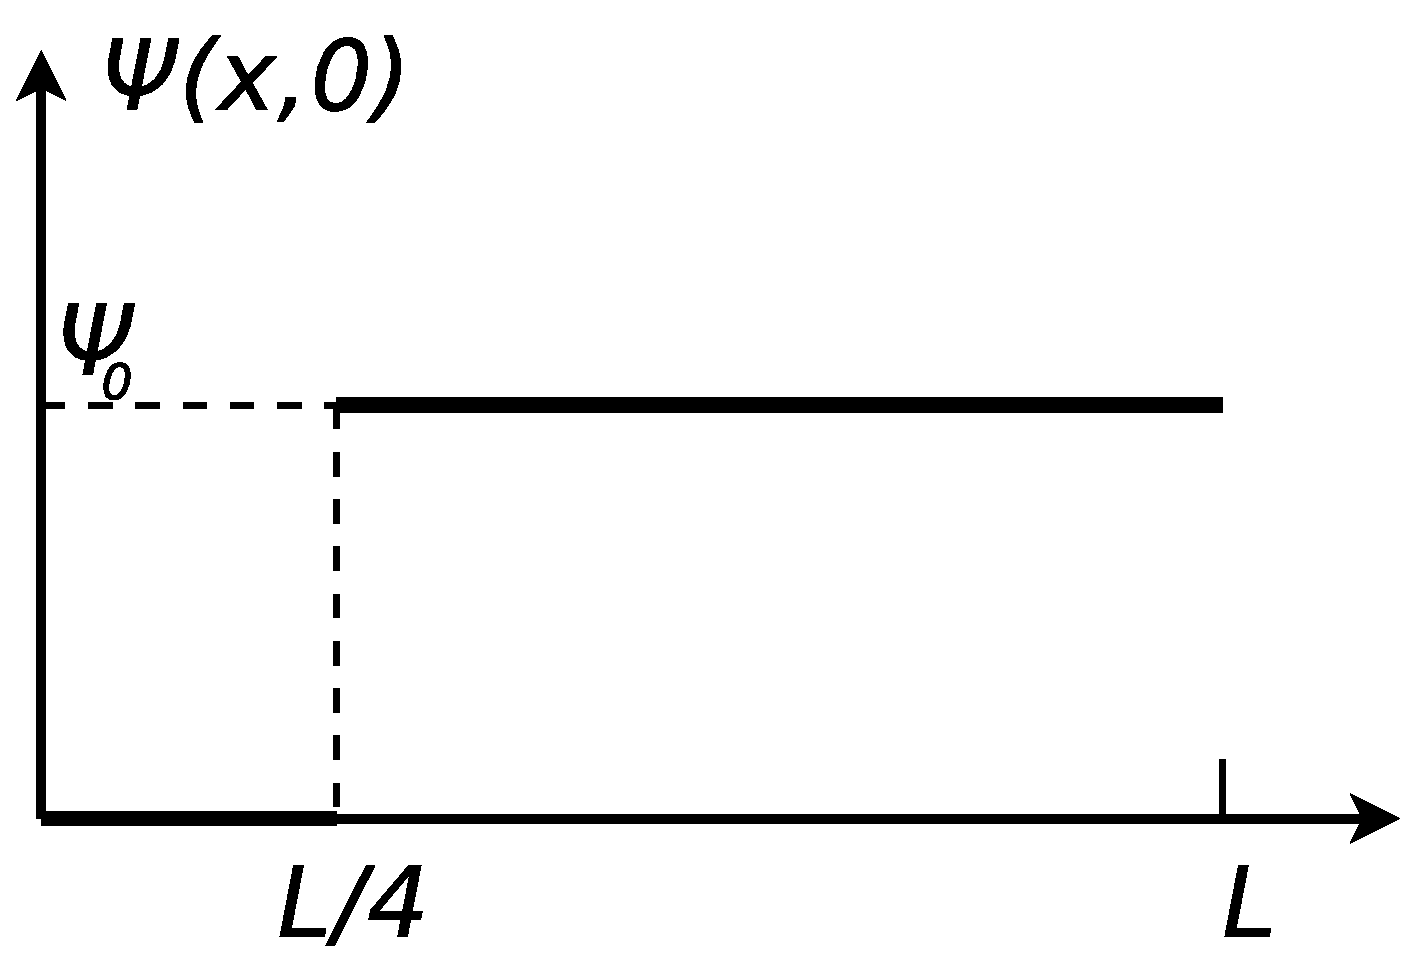
\includegraphics[clip,scale=0.25]{ej1-25}
\end{figure}

 

% \subsection*{Relación de disepersión en una cuerda}

\begin{enumerate}
\item Usando el sistema de coordenadas indicado en la figura, halle $\Psi(x,t)$.
\item Graficar $\Psi(x,t)$ para $\omega_{1}t=0,\,\pi$ y $2\pi$.
\item Si tomara un sistema de coordenadas con el origen en el extremo libre
de la cuerda, diga qué es lo que cambiaría. ¿Es conveniente ese sistema?
\end{enumerate}


\item Considere una cuerda de longitud $L$, siendo $T_{0}$ su tensión
y $\mu_{0}$ su densidad lineal. Sea $\Phi(x,t)$ la elongación de
la cuerda.

\begin{enumerate}
\item Escriba la expresión más general que representa un modo normal en
dicha cuerda, es decir, la expresión más general de una onda estacionaria.
\item Sabiendo que la cuerda tiene un extremo libre y otro fijo, y que el
sistema de coordenadas con el que trabaja es tal que el extremo libre
está en $x=0$ y el extremo fijo está en $x=L$, imponga las condiciones
de contorno y determine las constantes pertinentes.
\item Usando la relación de dispersión, obtenga las posibles frecuencias
temporales $\nu_{n}$. 
\item Si $\Phi(x,0)=0$ y $\dot{\Phi}(x,0)=V_{0}\cos\left(\frac{3\pi}{2L}x\right)$,
siendo $0\le x\le L$, obtenga la amplitud y fase de cada modo y halle
$\Phi(x,t)$.
\end{enumerate}



\item Dada una cuerda de longitud $L$ y densidad de masa uniforme $\mu$,
sometida a una tensión $T_{0}$ con ambos extremos fijos, demostrar
que si $\Phi(x,0)$ y $\dot{\Phi}(x,0)$ son simétricas con respecto
al centro de la cuerda, los modos con números de onda $k_{p}=2p\pi/L$
no se excitan.
\item Considere una cuerda de longitud $L$ sujeta en ambos extremos y sometida
a una tensión $T_{0}$, que consta de dos tramos: uno de longitud
$L_{1}$ y densidad de masa uniforme $\mu_{1}$, y otro de longitud
$L_{2}$ y densidad de masa uniforme $\mu_{2}$.
\begin{enumerate}
\item Halle la expresión más general para un modo normal en dicha cuerda.
Plantee las condiciones de contorno y halle las condiciones que deben
cumplir los distintos parámetros.
\item Considere que $L_{1}=3L_{2}$ y que $\mu_{2}=9\mu_{1}$. Hallar los
modos normales en este caso.
\end{enumerate}


\item Se tiene una cuerda de longitud $L$ y densidad de masa uniforme $\mu$,
sometida a una tensión $T_{0}$ y fija en ambos extremos. Se tiene
además que una fuerza de amortiguamiento proporcional a la velocidad
de la cuerda actúa en cada punto de la misma. Hallar la forma más
general de $\Phi(x,t)$.


\subsection*{Serie de Fourier: condiciones iniciales para gas en un tubo}


\item Se tiene un tubo de longitud $L$ cerrado en ambos extremos como se
indica en la figura. El tubo presenta un tabique ubicado en la mitad
del mismo. De un lado del tabique hay un gas de densidad $\rho_{0}-\Delta$
y del otro lado hay un gas de densidad $\rho_{0}+\Delta$ (considere
$\Delta\ll\rho_{0}$). Todo el gas se encuentra en reposo. A $t=0$
se quita el tabique y se deja evolucionar al sistema.
\begin{figure}[H]
\centering{}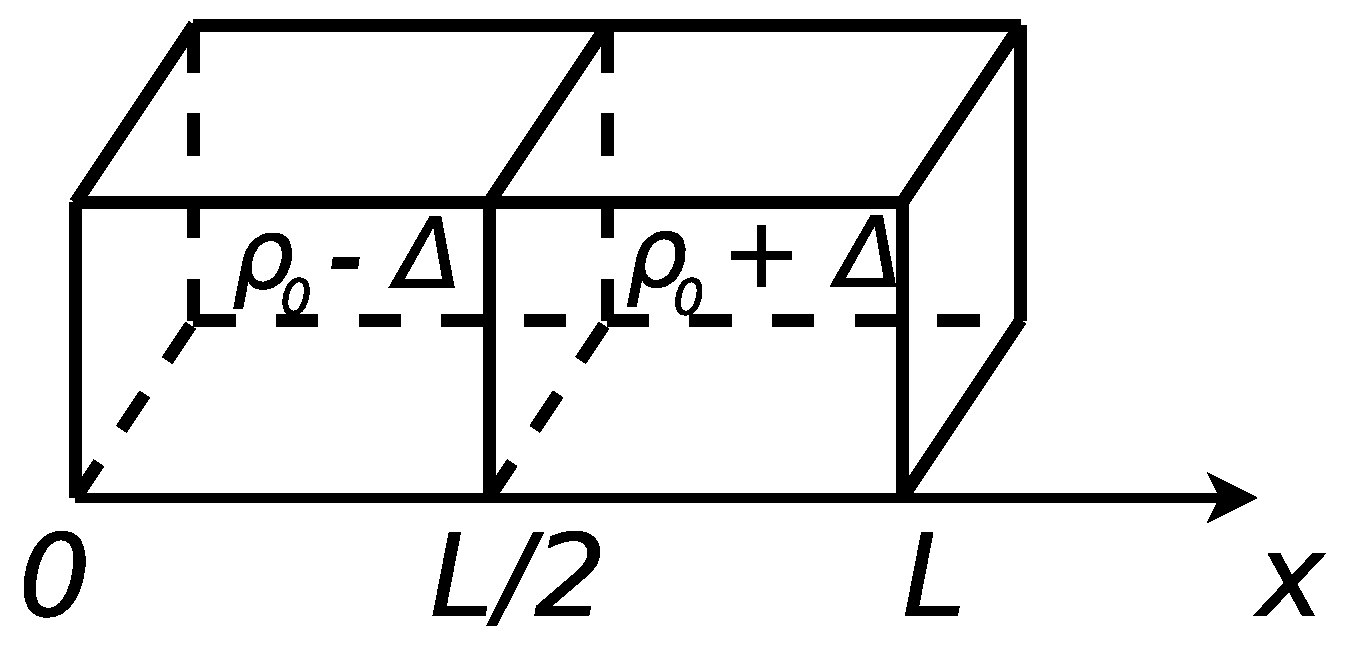
\includegraphics[clip,scale=0.25]{ej1-30}
\end{figure}


\begin{enumerate}
\item Escriba la expresión para un modo normal $\Psi_{n}(x,t)$ en el tubo,
imponiendo las condiciones de contorno. ¿Cuáles son las longitudes
de onda permitidas? ($\Psi$ es el desplazamiento de los elementos
del gas). 
\item Escriba la expresión de $\rho(x,0)$ y de $\Psi(x,0)$; grafíquelas.
Sugerencia: hallar $\Psi(x,0)$ a partir de $\rho(x,0)$ usando las
condiciones de contorno. 
\item Usando las condiciones iniciales, halle $\Psi(x,t)$. Calcule $\rho(x,0)$. \end{enumerate}
\begin{description}
\item [{Datos:}] $\rho_{0}$, $\Delta$, $L$, velocidad del sonido en
el gas $v_{s}$.
\end{description}
\item Se tiene un tubo dividido en dos regiones separadas por un tabique.
En una de ellas se tiene una presión $P=P_{0}+\Delta p$ (constante).
La otra región está abierta a la atmósfera, teniendo presión $P_{0}$.
A $t=0$ se remueve el tabique. Hallar $\delta p(x,t)$, $\Psi(x,t)$
y $\delta\rho(x,t)$.
\begin{figure}[H]
\centering{}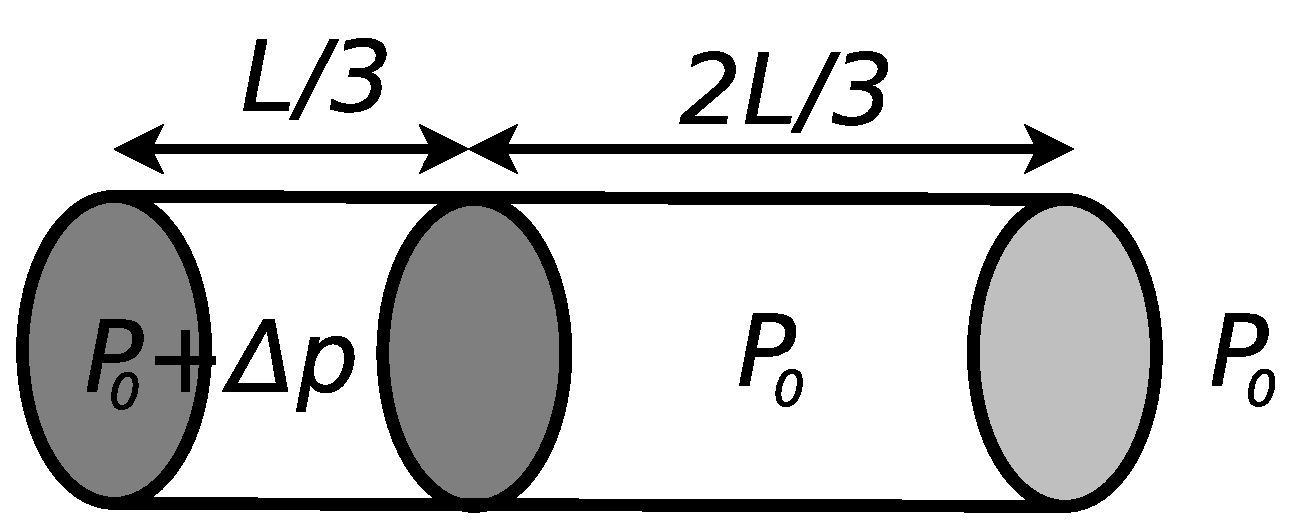
\includegraphics[clip,scale=0.25]{ej1-31}
\end{figure}
\begin{description}
\item [{Datos:}] $P_{0}$, $\Delta p\ll P_{0}$, $L$, $\gamma$ y la velocidad
del sonido en el gas $v_{s}$.
\end{description}


\subsection*{Onda estacionaria en cuerda como superposición de viajeras}


\item Se tiene una cuerda de longitud $L=0,6\unit{\, m}$, fija en sus dos
extremos, que se encuentra oscilando en uno de sus modos normales
como se muestra en la figura. La velocidad de propagación de las ondas
en dicha cuerda es \(v=80 \unit{m/s}\).
\begin{figure}[H]
\centering{}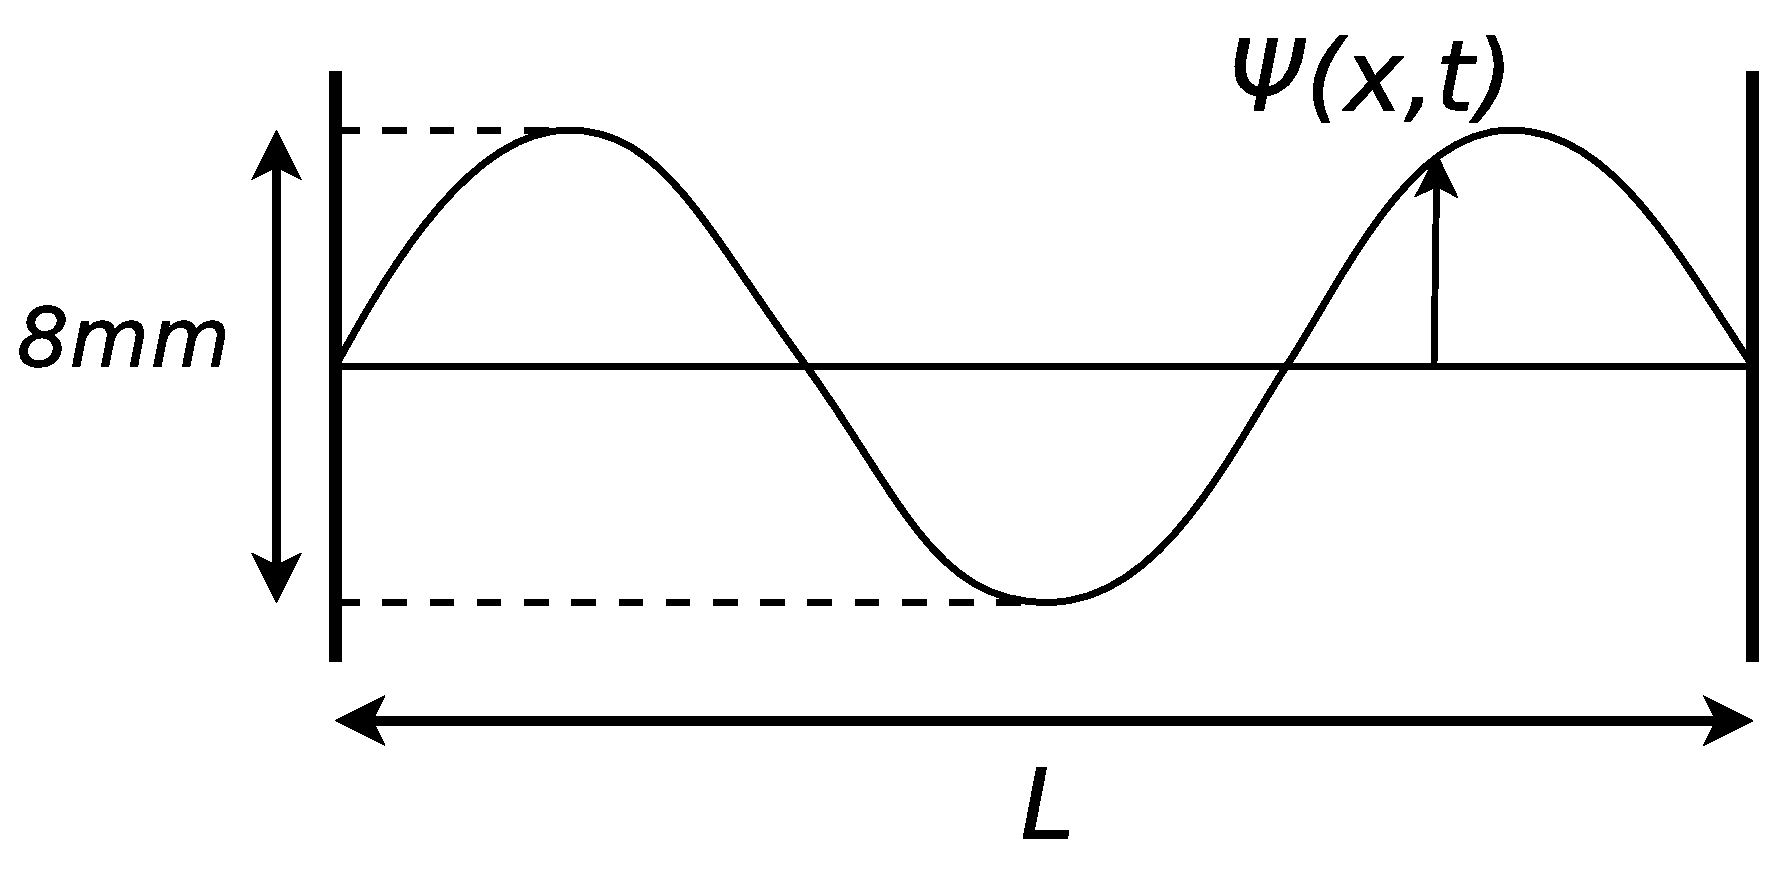
\includegraphics[clip,scale=0.25]{ej1-32}
\end{figure}
\begin{enumerate}
	\item Escribir $\Psi(x,t)$ (la elongación en un punto de la cuerda), sabiendo que a $t=0$ la elongación de todos los puntos es nula; que la amplitud total máxima de la onda es de \(8\unit{mm}\), y que $\dot{\Psi}(L/2,0)>0$
	\item Hallar $\Psi_{1}(x-vt)$ y $\Psi_{2}(x+vt)$ tales que $\Psi(x,t)=\Psi_{1}(x-vt)+\Psi_{2}(x+vt)$,
es decir: escribir a $\Psi(x,t)$ como la superposición de dos ondas
viajeras.
\end{enumerate}



\item Se tiene una cuerda de longitud $L=1\unit{m}$, con un extremo fijo y uno
libre, oscilando en el modo normal que se muestra en la figura. La
velocidad de propagación de las ondas en dicha cuerda es $v=80$\unit{m/s},
y el desplazamiento de las partículas a $t=0$ es el máximo posible
para este modo, siendo $\Psi(L,0)>0$. La amplitud total máxima es
de \SI{8}{mm}.
\begin{figure}[H]
\centering{}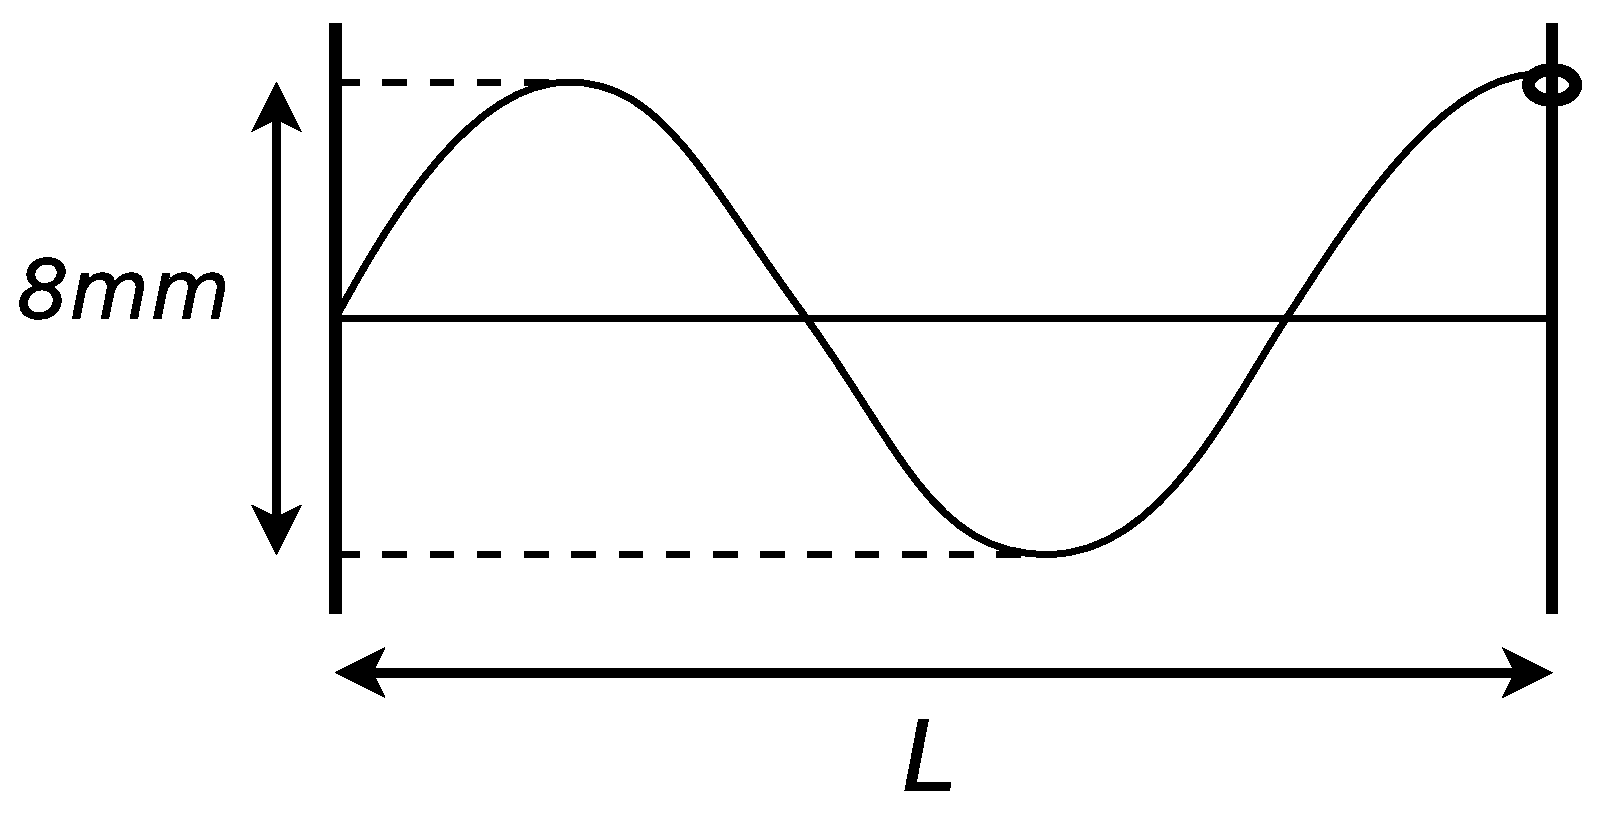
\includegraphics[clip,scale=0.25]{ej1-33}
\end{figure}
\begin{enumerate}
\item Resolver, para esta situación, todo lo pedido en el problema anterior. 
\item Si ahora la cuerda está oscilando en un modo normal arbitrario $n$,
con las mismas condiciones iniciales dadas arriba, repetir (a) (expresar
en función de $n$). \end{enumerate}
\end{enumerate}

\end{document}
